\documentclass[11pt,border=4pt]{standalone}
% Estilo comum dos fluxogramas do Caderno C3 (cores do modelo do MOP)
\usepackage[T1]{fontenc}
\usepackage[utf8]{inputenc}
\usepackage{helvet}
\renewcommand{\familydefault}{\sfdefault}
\usepackage{amssymb}
\usepackage{tikz}
\usetikzlibrary{positioning, arrows.meta, shapes.geometric, shapes.symbols, shapes.misc,
  calc, fit, backgrounds, decorations.pathmorphing, patterns, shadows}
% Paleta do modelo do caderno
\definecolor{cTeal}{HTML}{00747A}
\definecolor{cNavy}{HTML}{0B3A5A}
\definecolor{cBlue}{HTML}{0A73BA}
\definecolor{cBlueBg}{HTML}{EBF4F9}
\definecolor{cTealBg}{HTML}{E3F1F2}
\definecolor{cTealMid}{HTML}{9CCFD2}
\definecolor{cGrayBg}{HTML}{F2F2F2}
\definecolor{cGrayLine}{HTML}{BFBFBF}
\definecolor{cGrayText}{HTML}{595959}
\definecolor{cText}{HTML}{1A1A1A}
\definecolor{cAmber}{HTML}{B7791F}
\definecolor{cAmberBg}{HTML}{FDF3DC}
\definecolor{cGreen}{HTML}{3D7D3A}
\definecolor{cGreenBg}{HTML}{E8F2E4}
\color{cText}
\tikzset{
  every node/.style={font=\footnotesize, text=cText},
  etapa/.style={draw=cTeal, fill=cTealBg, rounded corners=2pt, align=center,
     inner sep=3.5pt, minimum height=0.85cm, text width=#1, line width=0.6pt},
  etapa/.default={3.2cm},
  marco/.style={draw=cNavy, fill=cNavy, rounded corners=2pt, align=center,
     inner sep=3.5pt, minimum height=0.85cm, text width=#1,
     font=\footnotesize\bfseries, text=white},
  marco/.default={3.2cm},
  marcoteal/.style={draw=cTeal, fill=cTeal, rounded corners=2pt, align=center,
     inner sep=3.5pt, minimum height=0.85cm, text width=#1,
     font=\footnotesize\bfseries, text=white},
  marcoteal/.default={3.2cm},
  externo/.style={draw=cGrayLine, fill=cGrayBg, rounded corners=2pt, align=center,
     inner sep=3.5pt, minimum height=0.85cm, text width=#1},
  externo/.default={3.2cm},
  produto/.style={draw=cTeal!70, fill=white, rounded corners=1pt, align=center,
     inner sep=2.5pt, minimum height=0.6cm, text width=#1, font=\scriptsize},
  produto/.default={2.4cm},
  decisao/.style={draw=cAmber, fill=cAmberBg, diamond, aspect=2, align=center,
     inner sep=1pt, font=\scriptsize, line width=0.6pt},
  correcao/.style={draw=cAmber, fill=cAmberBg, rounded corners=2pt, align=center,
     inner sep=3pt, minimum height=0.8cm, text width=#1, font=\scriptsize},
  correcao/.default={2.6cm},
  transversal/.style={draw=cBlue, fill=cBlueBg, dashed, rounded corners=2pt, align=center,
     inner sep=3.5pt, text width=#1, line width=0.6pt},
  transversal/.default={6cm},
  seta/.style={-{Stealth[length=2.2mm,width=1.8mm]}, line width=0.8pt, draw=cNavy},
  setaleve/.style={-{Stealth[length=1.8mm,width=1.5mm]}, line width=0.6pt, draw=cGrayText},
  setatracejada/.style={-{Stealth[length=2mm]}, line width=0.7pt, dashed, draw=cGrayText},
  rotulo/.style={font=\scriptsize\itshape, text=cGrayText, fill=white, inner sep=1pt},
  fase/.style={signal, signal to=east, signal from=west, draw=cTeal, fill=cTealBg,
     align=center, font=\scriptsize\bfseries, minimum height=1.05cm, text width=#1,
     inner sep=2pt},
  fase/.default={1.9cm},
  raia/.style={draw=cGrayLine, fill=cGrayBg, minimum width=#1, minimum height=0.9cm,
     anchor=north west},
  tituloraia/.style={font=\scriptsize\bfseries, text=cNavy, align=center, text width=1.75cm},
  cab/.style={font=\scriptsize\bfseries, text=white, fill=cNavy, align=center,
     inner sep=3pt, text width=#1, minimum height=0.6cm},
  cab/.default={3cm},
  bloco/.style={draw=cGrayLine, fill=cGrayBg, rounded corners=3pt},
}
% sem hifenização nas caixas dos fluxogramas
\AtBeginDocument{\hyphenpenalty=10000 \exhyphenpenalty=10000 \sloppy}

\begin{document}
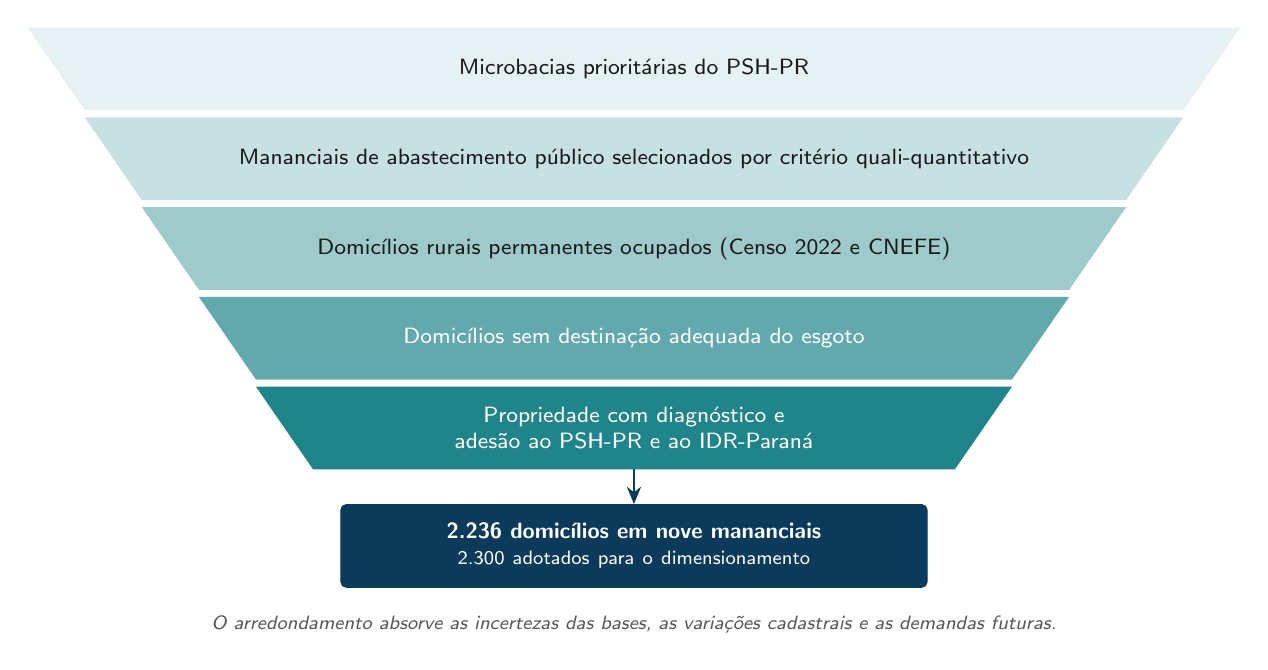
\begin{tikzpicture}[x=1cm,y=1cm]
  \fill[cTeal!10] (-7.7,0.0) -- (7.7,0.0) -- (6.9750000000000005,-1.05) -- (-6.9750000000000005,-1.05) -- cycle;
  \node[text width=12.68cm, align=center, font=\footnotesize, text=cText] at (0,-0.525) {Microbacias prioritárias do PSH-PR};
  \fill[cTeal!22] (-6.9750000000000005,-1.1400000000000001) -- (6.9750000000000005,-1.1400000000000001) -- (6.250000000000001,-2.1900000000000004) -- (-6.250000000000001,-2.1900000000000004) -- cycle;
  \node[text width=11.23cm, align=center, font=\footnotesize, text=cText] at (0,-1.665) {Mananciais de abastecimento público selecionados por critério quali-quantitativo};
  \fill[cTeal!38] (-6.25,-2.2800000000000002) -- (6.25,-2.2800000000000002) -- (5.525,-3.33) -- (-5.525,-3.33) -- cycle;
  \node[text width=9.78cm, align=center, font=\footnotesize, text=cText] at (0,-2.805) {Domicílios rurais permanentes ocupados (Censo 2022 e CNEFE)};
  \fill[cTeal!62] (-5.525,-3.4200000000000004) -- (5.525,-3.4200000000000004) -- (4.800000000000001,-4.470000000000001) -- (-4.800000000000001,-4.470000000000001) -- cycle;
  \node[text width=8.33cm, align=center, font=\footnotesize, text=white] at (0,-3.9450000000000003) {Domicílios sem destinação adequada do esgoto};
  \fill[cTeal!88] (-4.800000000000001,-4.5600000000000005) -- (4.800000000000001,-4.5600000000000005) -- (4.075000000000001,-5.61) -- (-4.075000000000001,-5.61) -- cycle;
  \node[text width=6.88cm, align=center, font=\footnotesize, text=white] at (0,-5.085000000000001) {Propriedade com diagnóstico e adesão ao PSH-PR e ao IDR-Paraná};
  \draw[seta] (0,-5.610000000000001) -- (0,-6.050000000000001);
  \node[marco=7.2cm, minimum height=1.05cm, anchor=north] at (0,-6.050000000000001) {2.236 domicílios em nove mananciais\\ \normalfont\scriptsize 2.300 adotados para o dimensionamento};
  \node[font=\scriptsize\itshape, text=cGrayText, anchor=north, text width=12cm, align=center] at (0,-7.350000000000001) {O arredondamento absorve as incertezas das bases, as variações cadastrais e as demandas futuras.};
\end{tikzpicture}
\end{document}
